% !TEX root = ../report.tex


\section{In-vehicle Communication Networks and Security}
\label{sec:communication-networks}

The different functions of a vehicle have very different requirements in
performance and safety needs. Therefor the quality of service needed from the
communication system varies (e.g. response time or bandwidth). Normally there
are different functional domains which divide the in-car embeeded systems
\cite{Navet2017}. There are the safety-critical domains "powertrain" (e.g.
engine control) and "chassis" (e.g. steering) that need a deterministic
real-time behavior. The functions of the "body" domain that controls for example
dashboard, wipers, lights and windows need to exchange many informations of
small size between each other. Other domains like "telematics" and "multimedia"
have for example increased requirements in bandwidth and confidentiality.

A multitude of different networks resulted out of this diversity of
requirements. Therefor the Society of Automotive Engineers (SAE) created in 1994
a classification for automotive communication protocols. This classification is
based on data transmision speed and functionality. There were 4 different
classes defined that are labeled class A to class D \cite{Ali2017}. Class A
networks have a speed lower than 10 kb/s. They are used for convenience features
such as trunk release or electric mirror adjustment. Examples for Class A
networks are LIN and TTP/A. Class B has a medium speed of 10 - 125 kb/s.
Networks of this classification are for general information between ECUs from
for example sensors. Main representatives of this class are J1850 and low-speed
CAN. High speed networks of class C have a speed between 125 kb/s and 1 Mb/s and
are used for real time control like the power train or vehicle dynamics.
High-speed CAN falls into this classification. Above the high speed
classification C there is class D. Every communication protocol faster than 1
Mb/s fall into this category. They are normally used either for multimedia
applications (e.g. MOST) or for hard real time critical functions like X-by-Wire
applications (e.g. TTP/C or FlexRay). Networks this fast, like FlexRay, can also
be used as gateways between sub-systems.

In modern vehicles it is normal that there are many networks of different types.
A BMW 7 series car from 2008 implements for example multiple LIN buses, a MOST
and a FlexRay bus and additionally four CAN buses \cite{Kellermann2008}. All of
these networks are normally interconnected by gateways.

TODO: Event-triggered versus Time-triggered

\subsection{CAN Network}

\subsection{Time-Triggered Networks}

\subsection{Low-Cost Automotive Networks}

\subsection{Multimedia and Infotainment Networks}

\subsection{Automotive Ethernet}

\subsection{Security Measures}

Controller Authentication, Encrypted Communication, Gateway
Firewalls \cite{Lemke2006}


\section{LeiA: Lightweight Authentication Protocol for CAN}
\label{sec:leia}

Overview of LeiA \cite{Radu2016}


\section{VatiCAN: Vetted, authenticated CAN bus}
\label{sec:vatican}

Overview of vatiCAN \cite{Nurnberger2016}

% \begin{figure}[h]
% 	\centering
% 	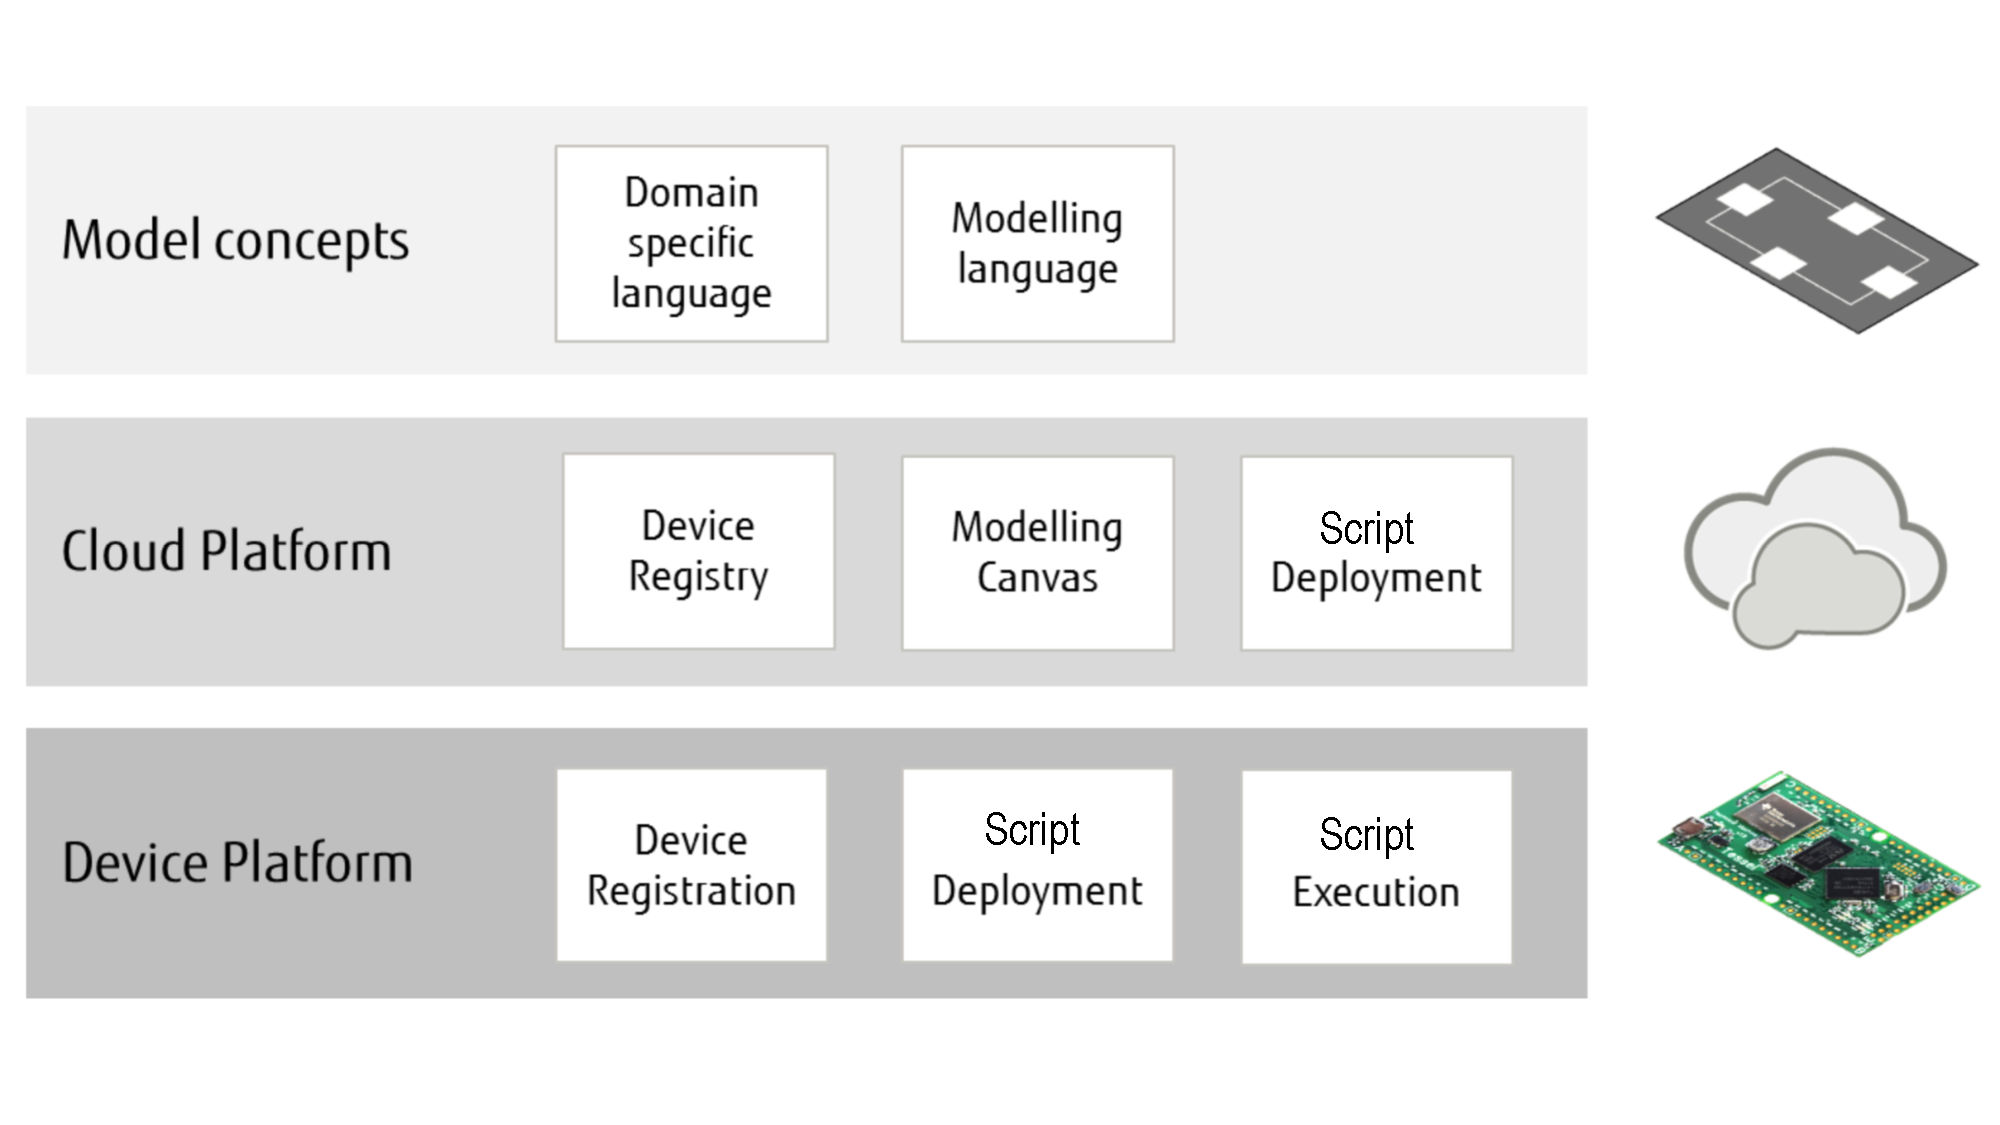
\includegraphics[width=0.8\linewidth]{Figures/sample-figure}
% 	\caption[]{Sample figure.}
% 	\label{fig:sample-figure}
% \end{figure}
